\chapter{Backend Implementation}

    \section{Architecture Overview}
        % Migrating from Express + MongoDB
        % Reasons: MapReduce in MongoDB has price of speed performance
        Before we choose Scalatra to be the server side of the system, we had been using Express\cite{expressjs} for the server and MongoDB\cite{mongodb} for the database. However, the reason why we migrate from this stack into Scalatra\cite{scalatra} is due to the performance of MapReduce in MongoDB. We use mapReduce database command for counting the number of people who has HIV, AIDS, TB, and STD disease in each case according to the requirements. MapReduce does not guarantee the speed of computation. It is not supposed to be used in the real time application. Moreover, as our system will contain more data, the speed performance will most likely to be dropped. This is the reason why we moved from Express and MongoDB stack into Scalatra for the backend.
        
    \section{Data Preprocessing}
    
        % ICT update data every 15 days via rsync command
        % It took a whole day since size of data is huge (1 TB)
        % contain irrelevant information (non-related visits)
        % 946 GB (from 2014 to now), Person: 421,444,580, Diagnosis: 1,423,970,811 record
        
        As we mentioned earlier in chapter \ref{section:how-the-data-flow} of how the data flow. First, ICT will update the data which is all the records of 43 health folders to our server in every 15 days by using rsync command. However, the process takes a whole day since the size of the data is 946 GB (since 2014 until 30 March 2017) which almost 1 TB. It contains 421,444,580 people and 1,423,970,811 diagnosis record which are include irrelevant information about the visits that do not have diseases under surveillance such as patient received paracetamol, vitamin C and etc. Within this size of data, our server will not be able to process all the data in reasonable duration of time. Therefore, we need to do multiple steps of data preprocessing before our data is ready for production.
        
        Let begin with when our server receive the data we need to create indexing to filtering our relevant 43 folder such as PERSON, LABFU, DIAGNOSIS{\_}IPD, DIAGNOSIS{\_}OPD, DRUG{\_}IPD, and DRUG{\_}OPD etc. Those indexing file create under the condition that those record are possible to relate to disease under surveillance. There are 4 indexing file that we create. First file is hp file where it store the hospcode and PID. Second file name hpa contain hospcode, PID and AN (admission number). Third file is hps which contain hospcode, PID, and SEQ. Last file is hn which contain hospcode and HN for our extra lab file because some lab file that upload to our system are not contain PID that use to be the linker of patient and lab result. Note that in this step we already get some filter raw file include LABFU, DIAGNOSIS{\_}IPD, DIAGNOSIS{\_}OPD, DRUG{\_}IPD, and DRUG{\_}OPD.
        
        After we create indexing file, now we go in to the process of filtering where the size of data will going to be reduce. We filter all relevant 43 folder using the most appropriate indexing file we create in the previous step. First we use hp file to filter PERSON, DEATH, ADDRESS and PRENATAL folder. We use hpa file to filter ADMISSION folder and use hps to filter SERVICE folder to delete all unrelate case such as broken leg, headache and etc. We use hn file to link the patient and extra lab result together.
        In addition, doing the process of filtering out some data we also anonymize all the sensitive information including hash all CID (Citizen identification number), change birth date to the first day of the month like 25 June 1956 to become 1 June 1956 because we only need to age of the patient and remove all first name, last name and etc. At the end of this process the data size will reduce very much for exmple in PERSON folder from approximate 400 million people to around 1 million people.
        
        Next, we need to perform indexing the data by hash cid. Before this step, all the data is grouped by province. However, if we group the data by province, it will be way more difficult to follow up the patient how many hospitals he/she visit in time series. Therefore, we need to perform indexing every record of the data by hash cid. First, we create a large hashmap by using hospcode and pid as the key to look for hash cid in PERSON folder. After that, we put the hash cid as the first column in every health folders that we use. We also perform sorting the data by hash cid.

        To make our backend system be able to perform parallel processing task when receive such request, we create a virtual shard. First, we set a number of shards to be 256. Then, we iterate through each record of each person. Next, we check if the hash cid of that person modulo with number of shard (in this case, 256) equals to zero. If it is, we put the record of that person into that shard. By doing this, it will always guarantee that every record that belongs to one person will belong to exactly 1 shard. There will be no record of that person goes across the shard. By doing this, it will give us benefit of parallel processing.
        
        \FloatBarrier
            \begin{figure}[h!]
                \centering
                    % can use width=\linewidth
                	\includegraphics[width=\linewidth]{images/chapter-06/data_reduction.png}
                	\caption{Data Preprocessing Diagram}
                	\label{data_preprocessing}
            \end{figure}
        \FloatBarrier
    
    \section{Implementation}
    
        % \subsection{Skimming Data}
        %     Originally, all the data from 43 folders that we got from Information Technology and Communication Center (under Office of the Permanent Secretary, Ministry of Public Health) since 2014 has the size of the data  more than 900 Gigabytes. It includes all the cases that patient visit to the hospital such as broken leg, headache, HIV, etc. Hence, every cases except HIV, AIDS, TB, and STD is irrelevant to our system.
            
        %     We filtered out the data that is not related to our system, hashing the citizen id number (protecting the privacy of the person), and group the remaining data by the hash result. We also sorted the data by the hash result. Hence, the size of the data is reduced into less than four Gigabytes.
        %     % separate file and hash (group & sort)
        % \subsection{Filter Data From Client Request} \label{filter-data}
        %     First of all before we go through on how server side work, we will explain how each drop-down select works. There are four main type of drop-down select as shown below.
        %     \subsubsection{Nation Drop-Down}
    In the nation drop-down button as shown in figure \ref{figure-nation-drop-down}, if user choose one of the lists as shown in figure \ref{figure-nation-lists}, it will be sent the value to the server which that the server will pass the nation filter to match that which type that user choose. Then it will get the the code of the country such as Thailand is 099, Myanma is 048, Laso is 056, and Cambodia is 057, in order to correctly count people in each nation depending on the nation filter.
    
% Thai = 099
%   val MYANMA: String = "048"
%   val LAOS: String = "056"
%   val CAMBODIA: String = "057"

    \FloatBarrier
        \begin{figure}[h!]
            \centering
                % can use width=\linewidth
        		
\includegraphics[width=\linewidth]{images/chapter-06/nation-1.png}
            	\caption{Nation Drop-Down}
        		\label{figure-nation-drop-down}
        \end{figure}
    \FloatBarrier
    
    \FloatBarrier
        \begin{figure}[h!]
            \centering
                % can use width=\linewidth
        		
\includegraphics[width=\linewidth]{images/chapter-06/nation-2.png}
            	\caption{Nation Lists}
        		\label{figure-nation-lists}
        \end{figure}
    \FloatBarrier
    
\subsubsection{Time Drop-Down}  

    
    In time drop-down button as shown in figure \ref{figure-time-drop-down}, there are three different type of it that user can choose as shown in figure \ref{figure-time-lists}. First, if user chooses all, it means that the server will choose time at the beginning of the data until the end of the data. The beginning here mean the first date of the data and the 23:59 of the end of the data. Second, if user chooses time-interval as shown in figure \ref{figure-time-interval-drop-down}, it means the server will choose the first date of the starting month, and follow by the month and the year that user choose to be the starting date time. Then it will end up at the end date of that month, the month and year that user choose as shown in figure \ref{figure-time-interval-drop-down}Third, if user chooses cut-off time as shown in figure  \ref{figure-time-end-date-drop-down}, it means that the server will choose the starting date at the beginning of the data and it will end up at the end date of the month that user choose, month, and year that user choose as shown in figure \ref{figure-time-end-date-drop-down}. In addition, the beginning date means that will pick the start of the date. for example if user choose first month and 2017, it means that the server will choose 1/1/2017. Unlike the beginning date, the end date will choose the last first of the date that pick, for instance, if user choose end date as second month and 2017, the server will choose 31/1/2017 at time 23:59.9.
    

    \FloatBarrier
        \begin{figure}[h!]
            \centering
                % can use width=\linewidth
        		
\includegraphics[width=9cm]{images/chapter-06/time-all.png}
            	\caption{Time Drop-Down}
        		\label{figure-time-drop-down}
        \end{figure}
    \FloatBarrier
    
    \FloatBarrier
        \begin{figure}[h!]
            \centering
                % can use width=\linewidth
        		
\includegraphics[width=9cm]{images/chapter-06/time-lists.png}
            	\caption{Time Lists}
        		\label{figure-time-lists}
        \end{figure}
    \FloatBarrier
    
    \FloatBarrier
        \begin{figure}[h!]
            \centering
                % can use width=\linewidth
        		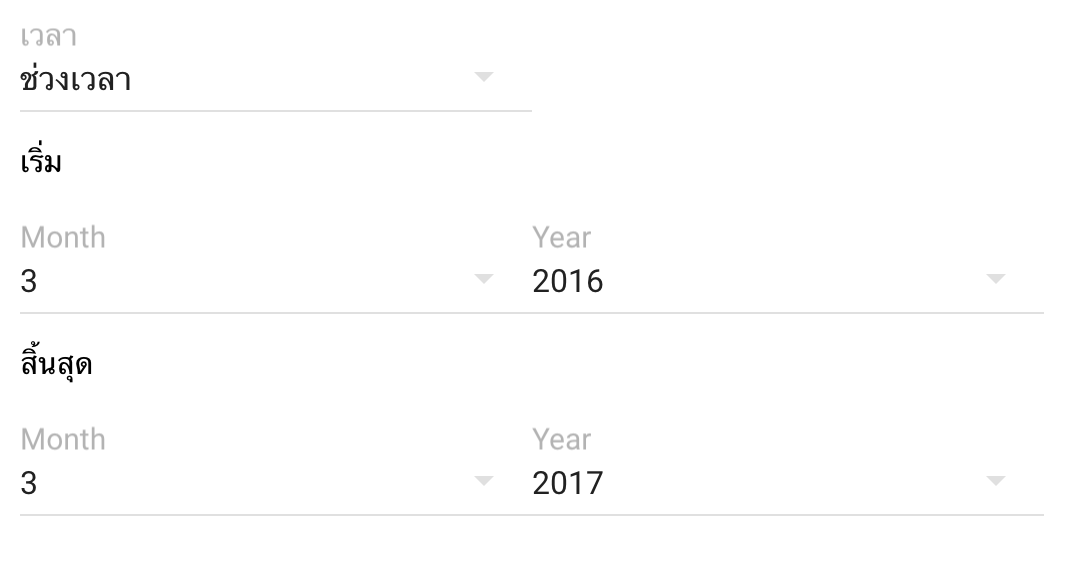
\includegraphics[width=\linewidth]{images/chapter-06/time-interval.png}
            	\caption{Time Interval Drop-Down}
        		\label{figure-time-interval-drop-down}
        \end{figure}
    \FloatBarrier
    
    \FloatBarrier
        \begin{figure}[h!]
            \centering
                % can use width=\linewidth
        		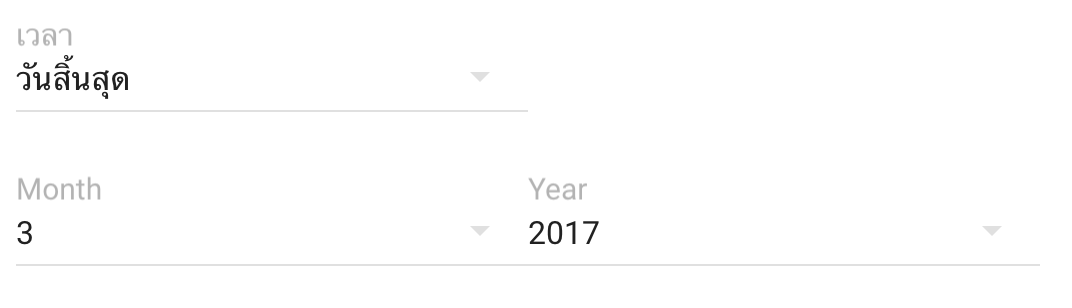
\includegraphics[width=\linewidth]{images/chapter-06/time-end-date.png}
            	\caption{Time End Date Drop-Down}
        		\label{figure-time-end-date-drop-down}
        \end{figure}
    \FloatBarrier
    
\subsubsection{Disease and Criteria Drop-Down}
    In disease and criteria drop-down button as shown in figure \ref{figure-disease-drop-down} and \ref{figure-disease-lists}, there are for different type of diseases that user can choose. Also in each disease there are many criteria that user can choose. It means that criteria will change according to the disease as shown in figure \ref{figure-disease-lists}. First, if user choose HIV, the criteria will show as in figure \ref{figure-disease-hiv-lists}, "All" means that choosing both HIV confirmed and HIV presumed. HIV confirmed means that patient who have diagnosis result (Z21, B20X, B21X) by the doctor and HIV presumed means that patient who receiving antiviral drug more than two types. "Confirmed" means choosing only HIV confirmed, and "HIV TB Comorbidity" means the server will choose patient that have HIV all and also the patient should have TB.
    % ?? "HIV TB" ==> which type of hiv(confirm or all)
    
    Second, if user choose Hepatitis C, the criteria will show as in figure \ref{figure-disease-hepatitis-c-lists}, "All" means choosing all patient that have diagnosis test in the criteria of hepatitis C. "Acute" means patient that has the diagnosis result of (B171, B1710, B1711) by the doctor and can be cured by the drug. "Chronic" means choosing the patient from the diagnosis result of (z2252,B182,B192,B1920,B1921) and this is the stage 2 that develop from acute if there is no drug action taken. It is when virus damages the liver enough to cause the signs and symptoms of liver disease. "Cirrhosis" means choosing the patient from the diagnosis result of (K743,K744,K745,K746) and have the previous diagnosis result in range of hepatitis C. Cirrhosis happen when the patient have permanent scar tissue replaces healthy liver cells from the virus of hepatitis C. "Hepatocellular Carcinoma" means the diagnosis result of the patient is C220 and have the previous diagnosis result in range of hepatitis C. It is a dead stage where patient need surgery as the hepatitis C virus developed to become the cancer.
    
    Third, if user choose Hepatitis B, the criteria will show as in figure \ref{figure-disease-hepatitis-d-lists}, All" means choosing all patient that have diagnosis test in the criteria of hepatitis B. "Acute" means choosing the patient that get the diagnosis result of (B160,B161,B162,B169) and can be cured by drug. "Chronic" means choosing the patient that has the diagnosis result of (Z2251,B180,B181,B191,B1910,B1911). Chronic hepatitis B is a development from acute stage of hepatitis B where there is no treatment taken place. "Acute With HDV" means the patient has the diagnosis of B160 or B161. It only happen to the patient who carry hepatitis B to be infect by HDV or Delta agent (Hepatitis D) and make the symptom of the patient get worse. "Chronic With HDV" means choosing the patient from the diagnosis result of B180 and the patient are infect to hepatitis D after carry the hepatitis B virus. "Cirrhosis" has the same diagnosis result as same as cirrhosis in hepatitis C but cause from the hepatitis B instead. "Hepatocellular Carcinoma" means choosing the patient diagnosis result of C220 and have the previous diagnosis result in the type of hepatitis B. It is the stage where the virus become cancer and patient need to surgery.
    
    Lastly, if user choose TB, There is only one criteria in this field which is "All". It means patient who have TB.
    
    
    \FloatBarrier
        \begin{figure}[h!]
            \centering
                % can use width=\linewidth
        		
\includegraphics[width=9cm]{images/chapter-06/disease.png}
            	\caption{Disease Drop-Down}
        		\label{figure-disease-drop-down}
        \end{figure}
    \FloatBarrier
    
    \FloatBarrier
        \begin{figure}[h!]
            \centering
                % can use width=\linewidth
        		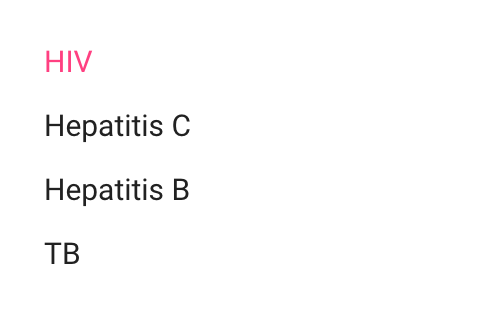
\includegraphics[width=9cm]{images/chapter-06/disease-lists.png}
            	\caption{Disease Lists}
        		\label{figure-disease-lists}
        \end{figure}
    \FloatBarrier
    
    \FloatBarrier
        \begin{figure}[h!]
            \centering
                % can use width=\linewidth
        		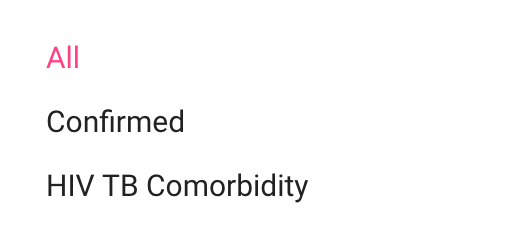
\includegraphics[width=9cm]{images/chapter-06/disease-hiv-lists.png}
            	\caption{HIV Lists}
        		\label{figure-disease-hiv-lists}
        \end{figure}
    \FloatBarrier
    
    \FloatBarrier
        \begin{figure}[h!]
            \centering
                % can use width=\linewidth
        		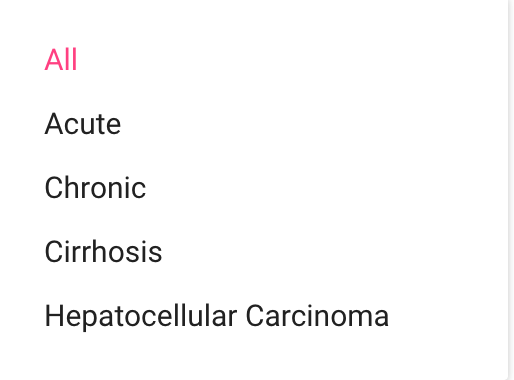
\includegraphics[width=9cm]{images/chapter-06/disease-hepatitis-c-lists.png}
            	\caption{Hepatitis C Lists}
        		\label{figure-disease-hepatitis-c-lists}
        \end{figure}
    \FloatBarrier
    
    \FloatBarrier
        \begin{figure}[h!]
            \centering
                % can use width=\linewidth
        		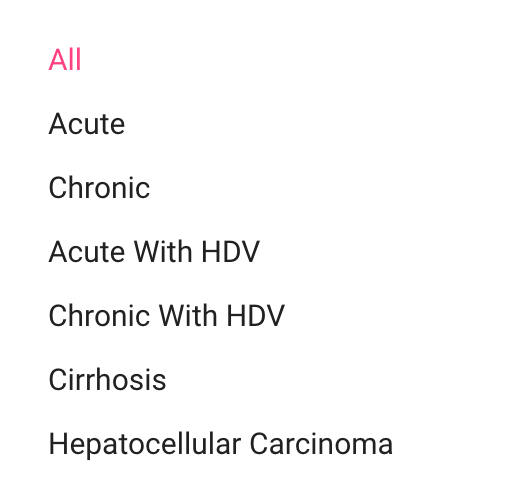
\includegraphics[width=8cm]{images/chapter-06/disease-hepatitis-d-lists.png}
            	\caption{Hepatitis B Lists}
        		\label{figure-disease-hepatitis-d-lists}
        \end{figure}
    \FloatBarrier


\subsubsection{Type of Report Dropdown}


    
    
    In type of report drop-down button as shown in figure \ref{figure-type-of-report-drop-down}, there are four different type of it that user can choose as shown in figure \ref{figure-type-of-report-lists}. First, if user chooses "Country", it means that the server will select all hospitals. Second, if user chooses "Area", it will pop-up area drop-down as shown in figure \ref{figure-type-of-report-area}, it means that the server will select the data according to the area that user choose. Third, if user chooses "Province" it will pop-up area drop-down and province drop-down  as shown in figure \ref{figure-type-of-report-province}, it means that the server will choose the data according to the province that user choose. Before user choose the province, the list of the province will be picked from the area that user choose. Lastly, if user chooses "Hospital" it will pop-up area drop-down, province drop-down, and hospital drop-down  as shown in figure \ref{figure-type-of-report-hospital}, it means that the server will choose the data according to the hospital that user choose. Like choosing "Province", the list of hospital will be picked from the province that user choose and the list of province will be picked according to the area that user choose.

    

    \FloatBarrier
        \begin{figure}[h!]
            \centering
                % can use width=\linewidth
        		
\includegraphics[width=9cm]{images/chapter-06/type-of-report-all.png}
            	\caption{Type of Report Drop-Down}
        		\label{figure-type-of-report-drop-down}
        \end{figure}
    \FloatBarrier
    
    \FloatBarrier
        \begin{figure}[h!]
            \centering
                % can use width=\linewidth
        		
\includegraphics[width=9cm]{images/chapter-06/type-of-report-lists.png}
            	\caption{Type of Report Lists}
        		\label{figure-type-of-report-lists}
        \end{figure}
    \FloatBarrier
    
    \FloatBarrier
        \begin{figure}[h!]
            \centering
                % can use width=\linewidth
        		
\includegraphics[width=\linewidth]{images/chapter-06/type-of-report-area.png}
            	\caption{Type of Report (Area Drop-Down)}
        		\label{figure-type-of-report-area}
        \end{figure}
    \FloatBarrier
    
    \FloatBarrier
        \begin{figure}[h!]
            \centering
                % can use width=\linewidth
        		
\includegraphics[width=\linewidth]{images/chapter-06/type-of-report-province.png}
            	\caption{Type of Report (Province Drop-Down)}
        		\label{figure-type-of-report-province}
        \end{figure}
    \FloatBarrier
    
    \FloatBarrier
        \begin{figure}[h!]
            \centering
                % can use width=\linewidth
        		
\includegraphics[width=\linewidth]{images/chapter-06/type-of-report-hospital.png}
            	\caption{Type of Report (Hospital Drop-Down)}
        		\label{figure-type-of-report-hospital}
        \end{figure}
    \FloatBarrier




    
        \subsection{At a Glance Report}\label{at_a_glance_report_back_end}
            As we know that we use POST method(for example, api/v1/hiv/at-a-glance/all) and pass it with body which contain all choose value that user choose in \ref{filter-data} then pass to the server. In server side, first it will filter by taking all the choose value to filter in order to make a correct structure and continue to do a map-reduce. After that it will return the json data to front-end.
            
            % all choose ==> filter ==> mapreduce ==> Json
        
        \subsection{Upload Lab File} \label{upload_file_back_end}
            % Only UPLOADER can upload lab file to the system
            The backend ensures that the user must have permission for uploading lab file into the server which mean the user must have "UPLOADER" role. Otherwise, it will reject by sending HTTP 401 status code (unauthorized). After the user uploaded the lab file, the server will response with total number of lines from the lab file, number of lines with correct format, number of lines with wrong format, and the lines with wrong format.
        
        \subsection{Checking Upload Lab File History Status }         \label{check_upload_history_status_ui_back_end}
            For this feature, every roles of the user can view the status of the uploaded lab files whether it has been uploaded or not during the selected year that user selected. When the user send the request, the server will return every hospitals within the province from the request and mark both in-patient lab file and out-patient lab file with boolean status whether that lab file has been uploaded to the system or not.
            
        
        \subsection{Demographics Report} \label{demographics_report_back_end}
            
            As we know that we use POST method(for example, /api/v1/hiv/demographic/all) and pass it with body which contain all choose value that user choose in \ref{filter-data} then pass to the server. In server side, first it will filter take all the choose value to filter in order to make a correct structure to continue to do a map-reduce. After that it will return the json data to front-end.
        % all choose ==> filter ==> mapreduce ==> Json
            
            
        % \subsection{Workload Report} \label{workload_report_backend}
        
        % \subsection{Individual Report}\label{individual_report_back_end}
        
        \subsection{Authentication}
            \subsubsection{Login}
                Authentication plays a major role in our system since the data is sensitive. We already create user accounts for all the users in our system. This means each hospital will have 1 account in our system. If the hospital's staff is changed, the account is still the same. If the user sign in successfully, we store the cookie into the browser. Otherwise, the server will return HTTP 401 status (unauthorized).
            \subsubsection{Logout}
                Once the user click logout on the web page, it will send the post request to /api/v1/auth/logout to the server. The server then will set the cookie to be expired and the user will need to login again to be able to interact with the system.
        
        
    \section{Unit Testing}
        We perform some unit testing on the backend since it defines the structural behavior of the system. There are some unit tests for API responses, authentication, model. We use ScalaTest\cite{scalatest} as our testing tool.

% multiple inheritance 

